%----------------------------------------------------------------------------------------
%	PACKAGES AND OTHER DOCUMENT CONFIGURATIONS
%----------------------------------------------------------------------------------------

\documentclass{beamer}

\usepackage[11pt,landscape,width=35.3,height=50,scale=0.4]{beamerposter}
\usepackage{mhchem}
\usepackage{subcaption}
\usepackage{bm}
\geometry{paperwidth=500mm,paperheight=353mm}

 % Use the beamerposter package for laying out the poster

\usetheme{confposter} % Use the confposter theme supplied with this template


%-----------------------------------------------------------
% Define the column widths and overall poster size
% To set effective sepwid, onecolwid and twocolwid values, first choose how many columns you want and how much separation you want between columns
% In this template, the separation width chosen is 0.024 of the paper width and a 4-column layout
% onecolwid should therefore be (1-(# of columns+1)*sepwid)/# of columns e.g. (1-(4+1)*0.024)/4 = 0.22
% Set twocolwid to be (2*onecolwid)+sepwid = 0.464
% Set threecolwid to be (3*onecolwid)+2*sepwid = 0.708

\newlength{\sepwid}
\newlength{\onecolwid}
\newlength{\twocolwid}
\newlength{\threecolwid}
\setlength{\sepwid}{0.025\paperwidth} % Separation width (white space) between columns
\setlength{\onecolwid}{0.3\paperwidth} % Width of one column
\setlength{\twocolwid}{0.464\paperwidth} % Width of two columns
\setlength{\threecolwid}{0.708\paperwidth} % Width of three columns
\setlength{\topmargin}{-0.5in} % Reduce the top margin size

\addtobeamertemplate{block end}{}{\vspace*{2ex}} % White space under blocks
\addtobeamertemplate{block alerted end}{}{\vspace*{2ex}} % White space under highlighted (alert) blocks

\setlength{\belowcaptionskip}{2ex} % White space under figures
\setlength\belowdisplayshortskip{2ex} % White space under equations



\setbeamercolor{block title}{fg=ngreen,bg=white} % Colors of the block titles
\setbeamercolor{block body}{fg=black,bg=white} % Colors of the body of blocks
\setbeamercolor{block alerted title}{fg=white,bg=dblue!70} % Colors of the highlighted block titles
\setbeamercolor{block alerted body}{fg=black,bg=dblue!10} % Colors of the body of highlighted blocks
% Many more colors are available for use in beamerthemeconfposter.sty
%-----------------------------------------------------------

\usepackage{graphicx}  % Required for including images

\usepackage{booktabs} % Top and bottom rules for tables

%----------------------------------------------------------------------------------------
%	TITLE SECTION 
%----------------------------------------------------------------------------------------

\title{Stochastic Networked SIS Disease Modelling} % Poster title

\author{Matthew Evans, supervised by Dr Andrew Krause} % Author(s)

\institute{Mathematical Sciences, Durham} % Institution(s)

%----------------------------------------------------------------------------------------

\begin{document}


\begin{frame}[t] % The whole poster is enclosed in one beamer frame

\begin{columns}[t] % The whole poster consists of three major columns, the second of which is split into two columns twice - the [t] option aligns each column's content to the top

\begin{column}{\sepwid}\end{column} % separator column

\begin{column}{\onecolwid} % The first column

%----------------------------------------------------------------------------------------
%	FIRST COLUMN
%----------------------------------------------------------------------------------------

\begin{alertblock}{Objectives}
Compartmental modelling is an old idea, first suggested by Kermack and Mckendrick in 1927\cite{kermackContributionMathematicalTheory1927}. Much of their techniques and analysis are still very relevant, though their model lacks a few critical elements. One of the greatest of these is the assumption that the population is continuous and homogeneous. This project aims to address these shortcomings by presenting two stochastic, discrete networked models of disease spread.
\end{alertblock}

\begin{block}{The Chemical SIS Model}

The population is divided into two compartments, Susceptible (S), or Infected (I). We then ascribe some dynamics to the system, describing the effect the number in each compartment has on the growth of the other. We treat the compartments as discrete, and treat the disease dynamics like chemical reactions

\begin{equation}
	\ce{S + I ->[k_I] 2 I} \qquad \ce{I ->[k_S] S}.
\end{equation}

We can then use the Gillespie SSA \cite{gillespieStochasticSimulationChemical2007} to simulate these reactions (see below), and can analyse them using a variety of well-developed tools, particularly the Chemical Master Equations (CMEs). These are a set of equations which tell us how the probability of there being a given number of infected people at a given time varies over time. For the non-networked SIS model, they are

\begin{align}
	\frac {\mathrm d} {\mathrm d t} P_n(t) &= k_S (n+1) P_{n+1}(t) + k_I (n-1)(N-(n-1)) P_{n-1}(t) \notag \\
	&\qquad - (k_S n + k_I n (N-n)) P_n(t).
\end{align}

We can also make the mass action approximation, that the rate of a reaction is proportional to the concentration of the reactants, giving us a simple ODE, which we can solve to get

\begin{eqnarray}
	I(t) = \frac {k_I N - k_S} {k_I + A \mathrm{exp}((k_S - k_I N) t)}.
\end{eqnarray}

Where $A$ is a constant specified by the initial condition.
\end{block}

\begin{figure}
	\centering
	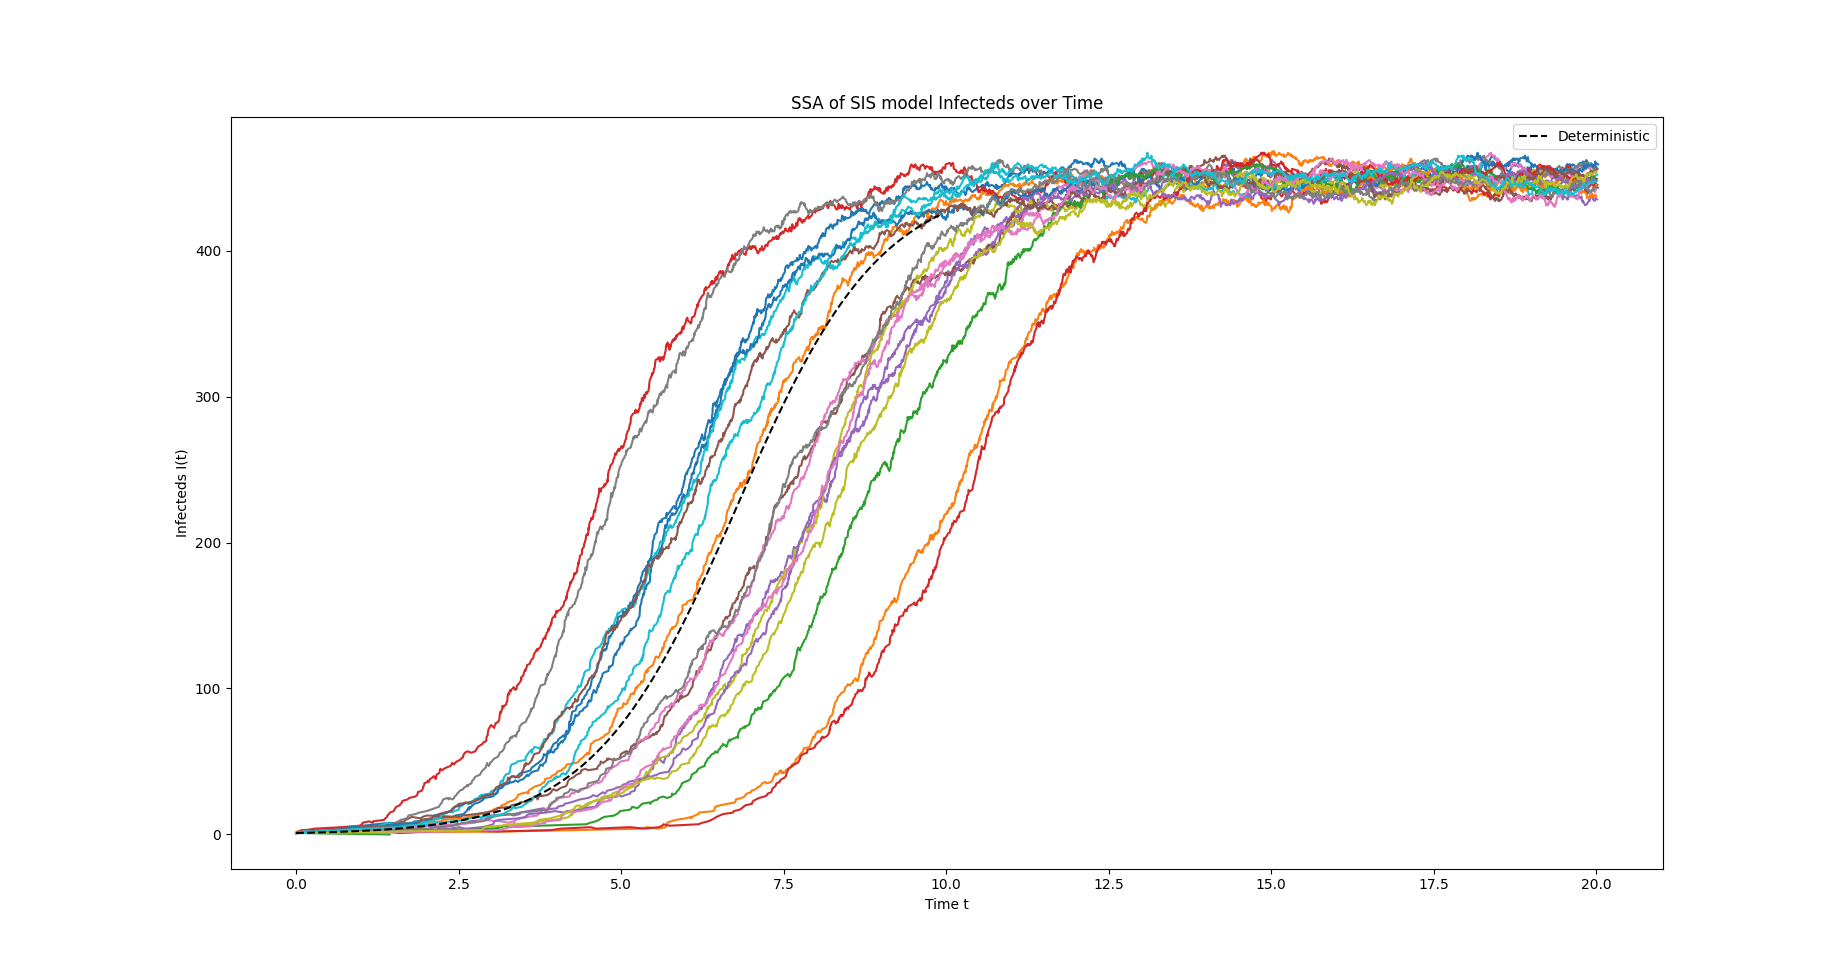
\includegraphics[width=\onecolwid] {figs/SISmix}
	\caption{A set of realisations of the Gillespie SSA on the well-mixed SIS model.}
\end{figure}

\end{column} % End of the first column

\begin{column}{\sepwid}\end{column} % Empty spacer column

\begin{column}{\onecolwid} % Begin a column which is two columns wide (column 2)

%----------------------------------------------------------------------------------------
%	MIDDLE COLUMN
%----------------------------------------------------------------------------------------

\begin{block}{Chemical SIS on Networks (Metapopulation)}

Our first approach to introducing spatial effects into the model is through a metapopulation approach, where we consider a simple graph and consider each node to have a population $N_i$, with $I_i(t)$ infected people. In our chemical approach, we treat infected and susceptible individuals from different nodes as being different "chemicals", giving the chemical equations

\begin{equation}
	\ce{I_i + S_i ->[k_I] 2 I_i} \qquad
	\ce{I_i ->[k_S] S_i} \qquad
	\ce{S_i + I_j ->[A_{ij} k_I] I_i + I_j}.
\end{equation}

The more complex system results in more unwieldy CMEs, though they are still of roughly the same form. However, we can gain some useful analytical insight by examining the mass action approximation

\begin{equation}
	\frac {\mathrm d I_i}{\mathrm d t} = k_I I_i(t) (N_i - I_i(t)) + k_I (N_i - I_i(t)) (\sum_j A_{ij} I_j(t)) - k_S I_i(t).
\end{equation}

If we then make the change to the continuous $\rho_i(t) = I_i(t) / N_i$, we can do some stability analysis and find that the extinction equilibrium does in fact become stable for sufficiently large $k_S$, or for very small populations $N$. We refer to this as the subcritical case. This stability analysis is done following the method in \cite{porterDynamicalSystemsNetworks2015}, where we seek the eigenvalues of the matrix $\bm{\mathsf{{M}}}$, given by

\begin{equation}
	M_{ij} = \delta_{ij} \left[ a_i + \sum_k b_{ik} A_{ij} \right] + c_{ij} A_{ij},
\end{equation}

where the coefficients are

\begin{align}
	a_i &:= k_I N_i (1 - 2 \rho_i^*(t)) - k_S, \\
	b_{ij} &:= -k_I N_i \rho_j^*(t), \\
	c_{ij} &:= k_I N_i (1 - \rho_i^*(t)).
\end{align}

We also find that a homogeneous ($\rho_i(t) = \rho$ for all $i$) equilibrium can exist provided the population satisfies certain properties. Crucially, for every node, the sum of its population with that of its neighbours must be the same.

\begin{figure}
	\centering
	\begin{subfigure}[t]{0.24\textwidth}
		\centering
		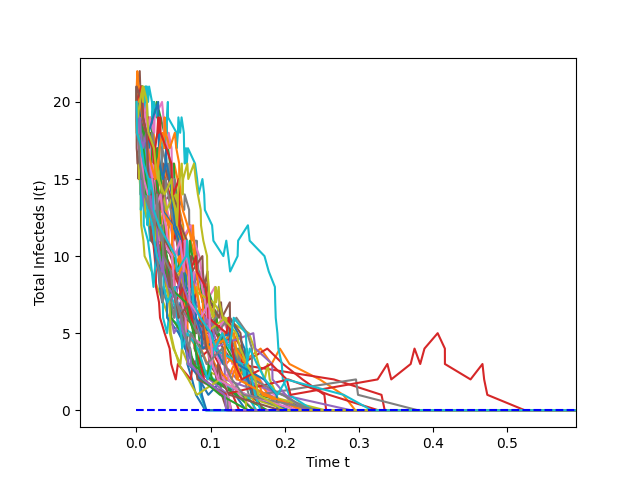
\includegraphics[width=\textwidth]{figs/SISmetak5sub.png}
		\caption{Subcritical $k_5$}
		\label{fig:SISmetak5sub}
	\end{subfigure}
	\begin{subfigure}[t]{0.24\textwidth}
		\centering
		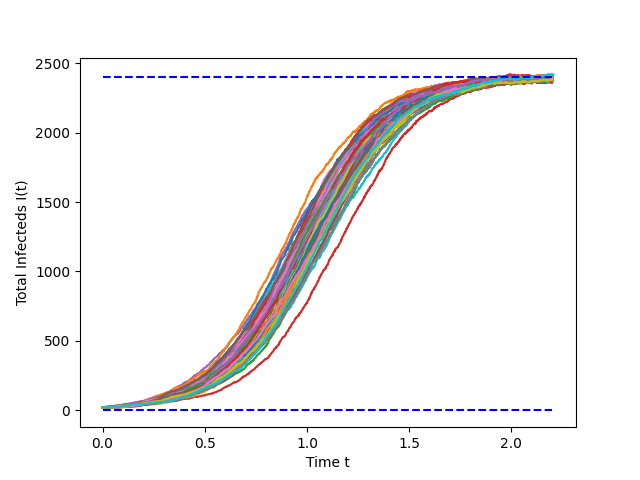
\includegraphics[width=\textwidth]{figs/SISmetak5sup.png}
		\caption{Supercritical $k_5$}
		\label{fig:SISmetak5sup}
	\end{subfigure}
	\begin{subfigure}[t]{0.24\textwidth}
		\centering
		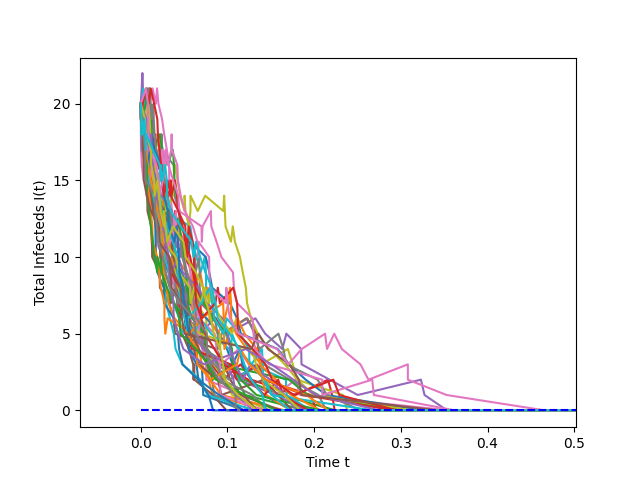
\includegraphics[width=\textwidth]{figs/SISmetaC5sub.png}
		\caption{Subcritical $C_5$}
		\label{fig:SISmetaC5sub}
	\end{subfigure}
	\begin{subfigure}[t]{0.24\textwidth}
		\centering
		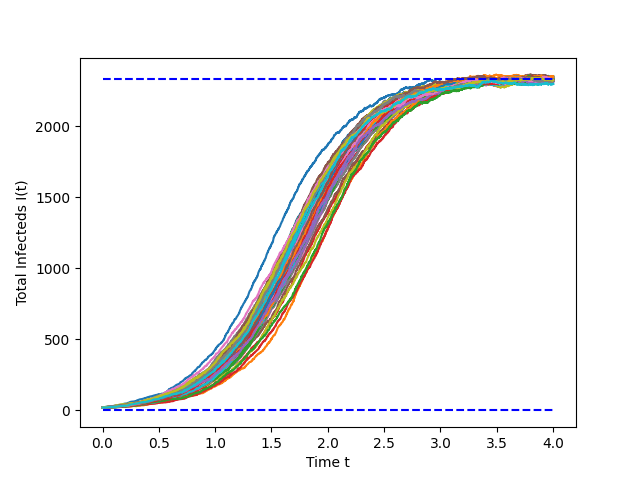
\includegraphics[width=\textwidth]{figs/SISmetaC5sup.png}
		\caption{Supercritical $C_5$}
		\label{fig:SISmetaC5sup}
	\end{subfigure}
	\begin{subfigure}[b]{0.24\textwidth}
		\centering
		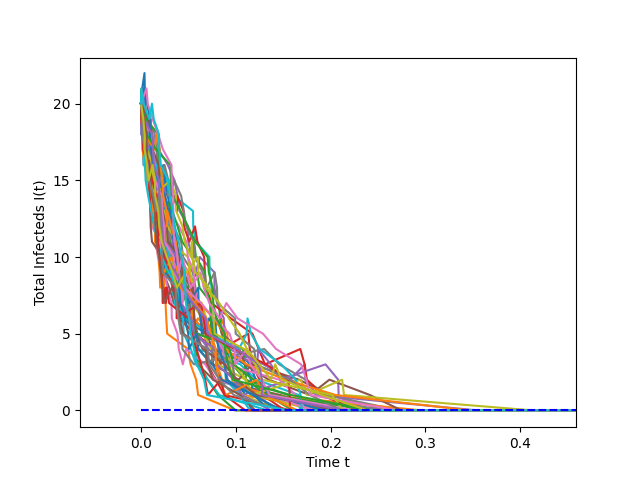
\includegraphics[width=\textwidth]{figs/SISmetaP5sub.png}
		\caption{Subcritical $P_5$}
		\label{fig:SISmetaP5sub}
	\end{subfigure}
	\begin{subfigure}[b]{0.24\textwidth}
		\centering
		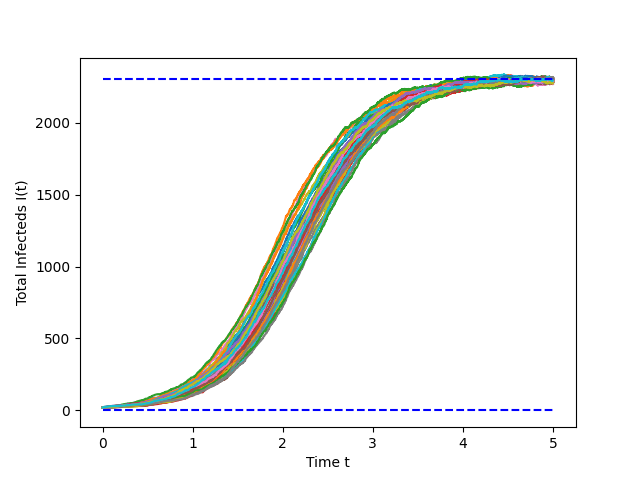
\includegraphics[width=\textwidth]{figs/SISmetaP5sup.png}
		\caption{Supercritical $P_5$}
		\label{fig:SISmetaP5sup}
	\end{subfigure}
	\begin{subfigure}[b]{0.24\textwidth}
		\centering
		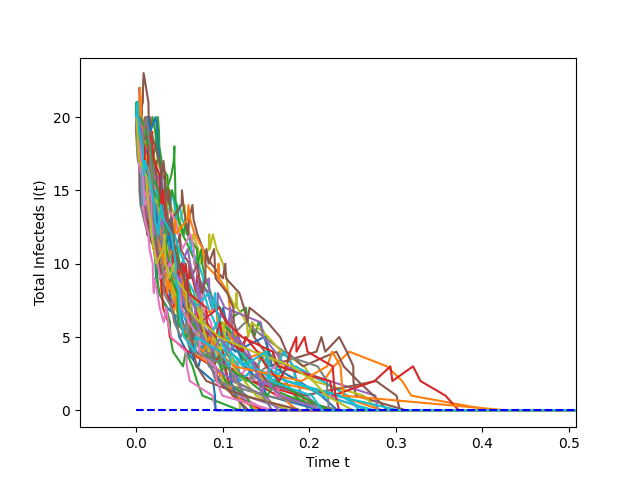
\includegraphics[width=\textwidth]{figs/SISmetaS4sub.png}
		\caption{Subcritical $S_4$}
		\label{fig:SISmetaS4sub}
	\end{subfigure}
	\begin{subfigure}[b]{0.24\textwidth}
		\centering
		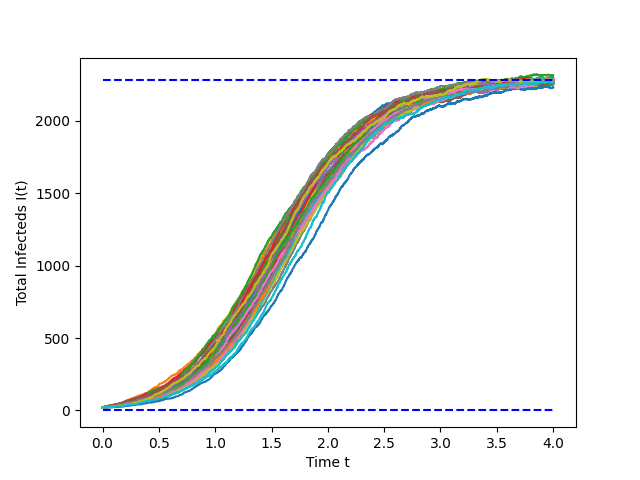
\includegraphics[width=\textwidth]{figs/SISmetaS4sup.png}
		\caption{Supercritical $S_4$}
		\label{fig:SISmetaS4sup}
	\end{subfigure}
	\label{figs:SISmeta}
\end{figure}

The above shows a set of realisations of the system using the Gillespie SSA, with parameters for the subcritical and supercritical regimes, on a variety of graphs. The populations were set to permit homogeneous equilibria on the graph, and the dotted blue lines show the extinction and (where it exists) the homogeneous endemic equilibria.

\end{block}

%----------------------------------------------------------------------------------------

\end{column} % End of the second column

\begin{column}{\sepwid}\end{column} % Empty spacer column

\begin{column}{\onecolwid} % The third column

%----------------------------------------------------------------------------------------
%	THIRD COLUMN
%----------------------------------------------------------------------------------------

\begin{block}{Chemical SIS on Networks (Individuals)}

Our final analysis uses much more complex graphs, but simply treats each node as an individual person. As there is no infection within a node, this actually simplifies the chemical equations once again, to

\begin{equation}
	\ce{S_i + I_j ->[A_{ij} k_I] 2 I} \qquad \ce{I_i ->[k_S] S_i}.
\end{equation}

We once again simulate this system using a (somewhat modified) Gillespie SSA. We also find that the CMEs can be written more simply, as

\begin{equation}
	\frac {\mathrm d p_i} {\mathrm d t} = k_I \sum_j A_{ij} p_j(t) - \left( k_I \sum_j A_{ij} p_j(t) + k_S \right) p_i(t).
\end{equation}

Where $p_i(t)$ represents the probability of node $i$ being infected at time $t$. We then examine the behvaiour on a variety of graphs, both simple and more complex. Particularly, we look at several random graphs such as the Erdos-Renyi, Watts-Strogatz, Barabasi-Albert, and bond percolation graphs. These all have characteristics of real-world social networks, but also have a variety of limitations. However, we also obtained a data set of $4000$ facebook users and their connections from the SNAP dataset \cite{snapnets}, which we were able to use to simulate the disease spread. The resulting trajectories, as well as an image of the graph part-way through the epidemic, are below.

\begin{figure}
	\centering
	\begin{subfigure}{0.45\textwidth}
		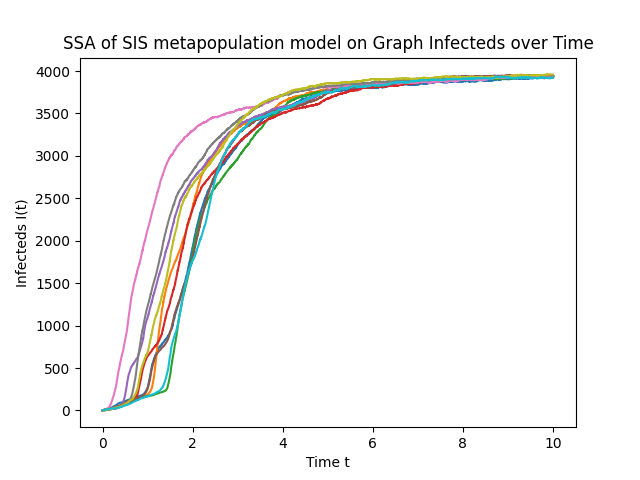
\includegraphics[width=\textwidth]{figs/facebook_curves.png}	
	\end{subfigure}
	\begin{subfigure}{0.45\textwidth}
		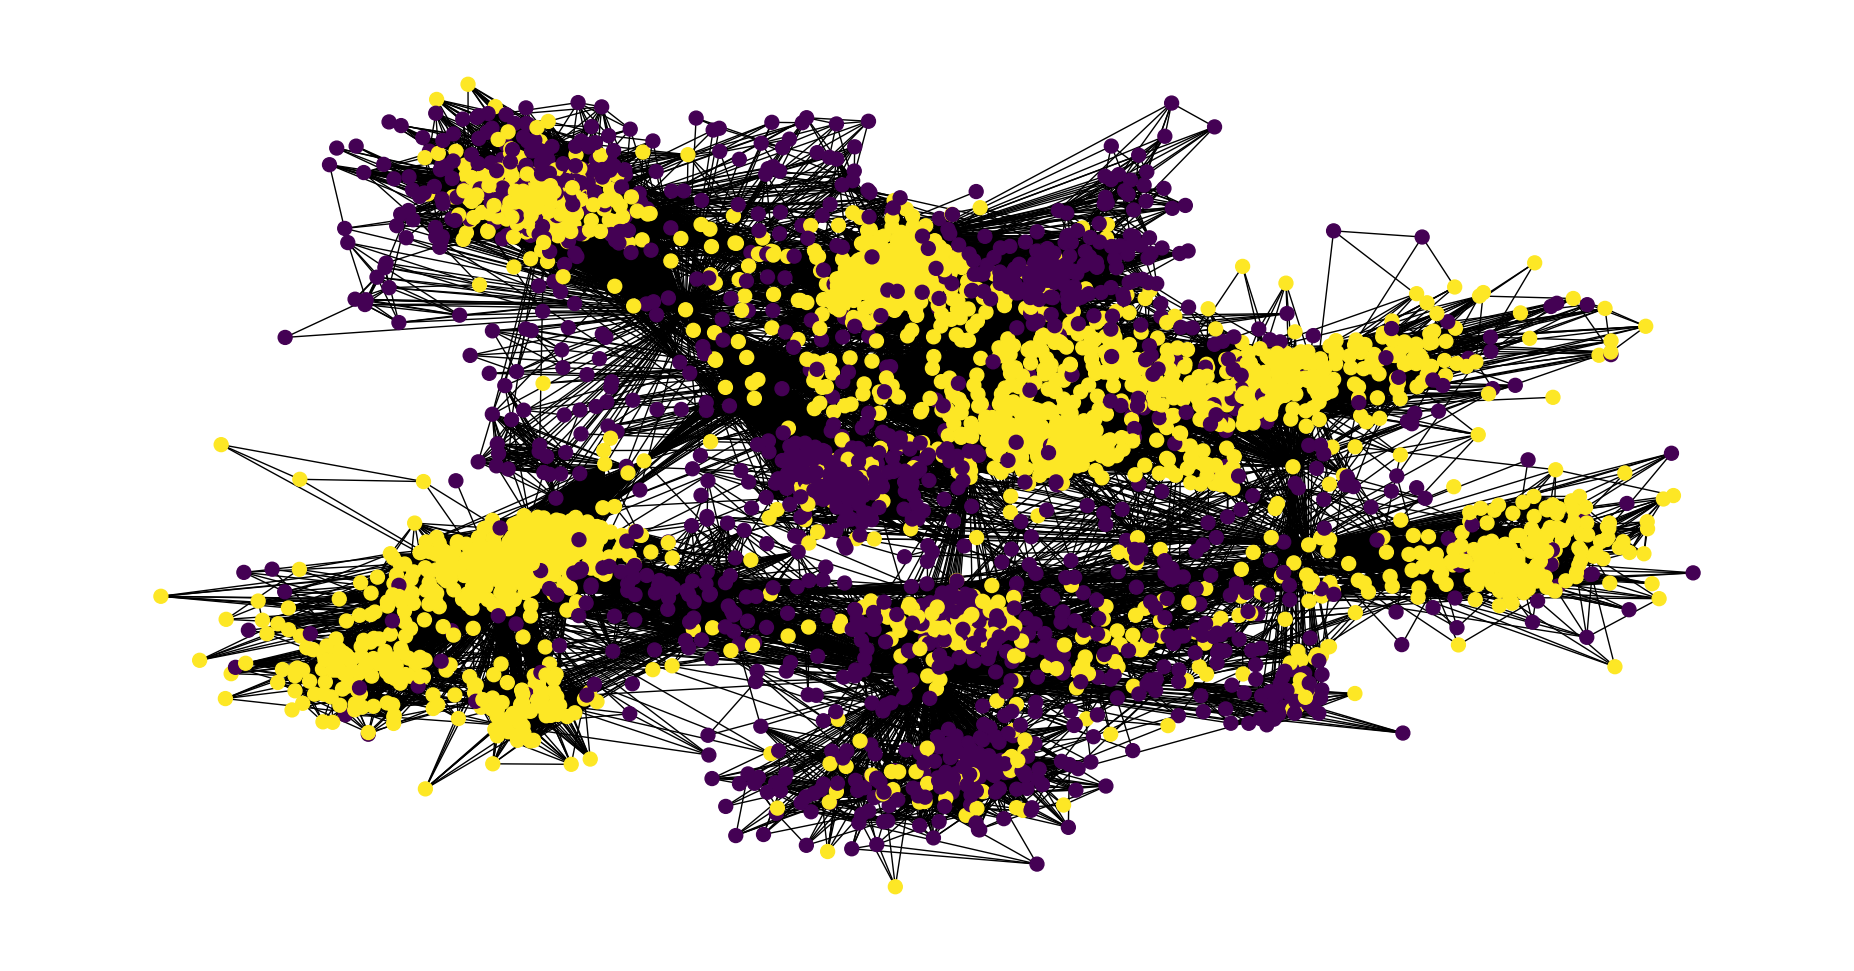
\includegraphics[width=\textwidth]{figs/facebook_partway.png}
	\end{subfigure}
\end{figure}

\end{block}

\begin{alertblock}{References}
\small{\bibliographystyle{unsrt}
\bibliography{mybib}}
\end{alertblock}

%----------------------------------------------------------------------------------------

\end{column} % End of the third column

\begin{column}{\sepwid}\end{column} % separator column

\end{columns} % End of all the columns in the poster

\end{frame} 
% End of the enclosing frame

\end{document}
